\section{Conception et réalisation}

\subsection{Partir de l'utilisateur}

En premier lieu il nous a semblé intéressant de s'imaginer le comportement d'un utilisateur devant le programme fini. Ainsi, au fil des actions du personnage virtuel,
l'allure globale du projet se détaille.  

Le schéma d'utilisation classique part d'une importation d'un ensemble de dossiers ou fichiers de type Open Document Text ( abrégé ODT par la suite ) . Dès lors se posent évidemment les questions de recherche et vérification de type des fichiers : Une validation par MIME-Type est préférée à la classique comparaison de l'extension.

Après l'importation vient l'extraction des données à analyser ensuite : Sur ce point nous avons eu de nombreuses discussions, notamment sur l'automatisation de cette tâche.
% \subsection{Une sous section}

% On peut mettre des mots en \emph{italique}, 
% en \textsc{petites Majuscules} ou 
% en \texttt{largeur fixe (machine à écrire)}.

% Voici un deuxième paragraphe avec une formule mathématique simple : $e = mc^2$.

% Un troisième avec des \og guillemet français \fg{}.

% \subsubsection{Écrire en anglais}

% \foreignlanguage{english}{Do you speak French? Does anybody here speak french?}


% \subsection{Lites}

% \begin{itemize}
% \item Liste classique ;
% \item un élément ;
% \item et un autre élément.
% \end{itemize}
% \vspace{\parskip} % espace entre paragraphes

% \begin{enumerate}
% \item Une liste numéroté
% \item deux
% \item trois
% \end{enumerate}
% \vspace{\parskip}

% \begin{description}
% \item[Description] C'est bien pour des définitions.
% \item[Deux] Ou pour faire un liste spéciale.
% \end{description}
% \vspace{\parskip}


% \subsection{Références}

% Voici une référence à l'image de la figure \ref{bloghiko} page \pageref{bloghiko} et une autre vers la partie \ref{p2} page \pageref{p2}.

% On peut citer un livre\,\up{\cite{lpp}} et on précise les détails à la fin du rapport dans la partie références.


% \subsection{Note de bas de page}

% Voici une note\,\footnote{Texte de bas de page} de bas de page.
% Une deuxième\,\footnotemark{} déclarée différemment.
% La même note\,\footnotemark[\value{footnote}].

% \footnotetext{Il a deux références vers cette note}


% \subsection{Figure}

% \begin{figure}[!ht]
%     \center
%     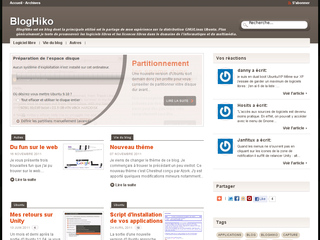
\includegraphics[]{./images/bloghiko.jpg}
%     \caption{BlogHiko | taille original}
%     \label{bloghiko}
% \end{figure}

% \begin{figure}[!ht]
%     \center
%     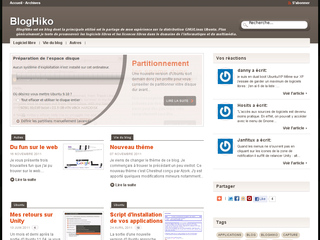
\includegraphics[width=0.5\textwidth]{./images/bloghiko.jpg}
%     \caption{BlogHiko | 50\% de la largeur de la page}
% \end{figure}


